\documentclass{beamer}


      \mode<presentation>

      \usetheme{Warsaw}

      \usecolortheme{lily}

\usebackgroundtemplate{
\includegraphics[width=\paperwidth]{format/libresoft-bg-soft.png}}
      \beamertemplateballitem

      \setbeameroption{show notes}
      \usepackage[utf8]{inputenc}

      \usepackage[T1]{fontenc}

      \usepackage{hyperref}

      \usepackage{color}
      \usepackage{listings}
      \lstset{numbers=none,language=[ISO]C++,tabsize=4,
  frame=single,
  basicstyle=\small,
  showspaces=false,showstringspaces=false,
  showtabs=false,
  keywordstyle=\color{blue}\bfseries,
  commentstyle=\color{red},
  }

      \usepackage{verbatim}

\usepackage[english]{babel}
\usepackage[utf8]{inputenc}
\usepackage{times}
\usepackage[T1]{fontenc}
\usepackage{graphics}

\title{Development of Libre Software}
\subtitle{}
\author{Carlos García Campos \\{\it cgarcia@igalia.com}}
\institute{}
\date{}

\begin{document}

\begin{frame}
\titlepage
\end{frame}

%\section{Python}

\begin{frame}
  \frametitle{Introduction}

  \begin{itemize}
  \item High level interpreted language created by Guido van Rossum
  \item First public release in 1991
  \item Designed to be simple to use
  \item Readability
  \item Object Oriented
  \item ``Multiplatform''
  \item The interpreter is extensible (written in C)
  \item Free Software!
  \end{itemize}
\end{frame}

\begin{frame}
  \frametitle{History}

  \begin{itemize}
  \item In the early 80s, Guido van Rossum worked at CWI (Centrum voor
    Wiskunde \& Informatica) in Netherlands, developing the ABC
    programming language.
  \item In 1986 van Rossum is moved to a different project, the Amoeba
    project, a distributed operating system.
  \item By the late 80s they realized they need and scripting language
    for Amoeba, and Guido started to work on his own programming
    language (in his free time taking advantage of the Christmas holidays)
  \item During 1990 he continued working on Python in his own time.
  \item In February 1991 the 0.9 version is released.
  \item The version 1.0 is released in January 1994.
  \end{itemize}
\end{frame}

\begin{frame}
  \frametitle{History (Cont.)}

  \begin{itemize}
  \item In 1995 Guido van Rossum leaves CWI and moves to Corporation
    for National Research Initiatives (CNRI) in Reston, Virginia where
    he continues developing Python.
  \item In 2000, the Python core development team moved to BeOpen.com
    to form the BeOpen PythonLabs team.
  \item In October 2000 version 2.0 is released by BeOpen.com
  \item After 2.0 was released, the PythonLabs developers joined
    Digital Creations (later renamed as Zope Coorporation)
  \item In March 2001, the Python Software Foundation (PSF) is founded
    as a non-profit organization in order to protect and promote the
    Python development.
  \item Today, the project has an important community around and
    Python is the language selected by many different projects.
  \item Python 3.0 (a.k.a Python 3000) is the latest major release 
    and it breaks backwards compatibility with Python 2.
  \end{itemize}
\end{frame}

\begin{frame}[fragile]
  \frametitle{Hello World}
{\huge
\begin{verbatim}
print "Hello World"
\end{verbatim}
}
\end{frame}

\begin{frame}[fragile]
  \frametitle{The interpreter}

  \begin{itemize}
  \item Interactive mode
{\scriptsize
\begin{verbatim}
Python 2.5.2 (r252:60911, Oct  5 2008, 19:24:49) 
[GCC 4.3.2] on linux2
Type "help", "copyright", "credits" or "license" for more information.
>>> 2 + 2
4
>>> print "Hello World"
Hello World
>>>
\end{verbatim}
}
\item Running scripts
{\scriptsize
\begin{verbatim}
#!/usr/bin/env python

print "Hello World"
\end{verbatim}
}

\item ipython: An Enhanced Interactive Python
\end{itemize}
\end{frame}

\begin{frame}
  \frametitle{Builtin data types}
  \begin{itemize}
  \item Elemental types: int, float, bool, long, ...
  \item Strings: str, unicode
  \item Compound types: list, tuple, dict, ...
  \end{itemize}
\end{frame}

\begin{frame}[fragile]
  \frametitle{Strings}
  \begin{itemize}
  \item Single or double quotes
{\scriptsize
\begin{verbatim}
>>> "double quote" == 'double quote'
True
>>> 'single \' quote'
"single ' quote"
>>> "single ' quote"
"single ' quote"
\end{verbatim}
}

\item Even triple quotes: """ or '''
{\scriptsize
\begin{verbatim}
>>> print "We need to scape\n\
... new lines"
We need to scape
new lines
>>> print """No need to scape
... new lines"""
No need to scape
new lines
\end{verbatim}
}  

\item Raw string
{\scriptsize
\begin{verbatim}
>>> print "Not\t a raw\n string"
Not a raw
 string
>>> print r"It's\t a raw\n string"
It's\t a raw\n string
\end{verbatim}
}
\end{itemize}
\end{frame}

\begin{frame}[fragile]
  \frametitle{Strings (Cont.)}
  \begin{itemize}
  \item Concatenate and repeat
{\scriptsize
\begin{verbatim}
>>> "Hello" + "World"
'HelloWorld'
>>> "Hello"*5
'HelloHelloHelloHelloHello'
\end{verbatim}
}

\item Indexing
{\scriptsize
\begin{verbatim}
>>> s = "Hello World"
>>> s[6]
'W'
\end{verbatim}
}

\item Unicode
{\scriptsize
\begin{verbatim}
>>> print u'Danke schön für alles!'
Danke schön für alles!
>>> u'Danke schön für alles!'
u'Danke sch\xf6n f\xfcr alles!'
>>> print u'Danke sch\xf6n f\xfcr alles!'
Danke schön für alles!
>>> print 'Danke sch\xf6n f\xfcr alles!'
Danke schn fr alles!
\end{verbatim}
}

\end{itemize}
\end{frame}

\begin{frame}[fragile]
  \frametitle{Lists and tuples}
  \begin{itemize}
  \item Ordered sequence of items
{\scriptsize
\begin{verbatim}
>>> ['string', 5.0, u'unicode', 2, ['a', "b"], r'raw']
['string', 5.0, u'unicode', 2, ['a', 'b'], 'raw']
\end{verbatim}
}

\item Indexing
{\scriptsize
\begin{verbatim}
>>> print l[0], l[-1], l[-2]
string raw ['a', 'b']
>>> print l[3:], l[:3], l[:-4]
[2, ['a', 'b'], 'raw'] ['string', 5.0, u'unicode'] ['string', 5.0]
>>> print l[:]
['string', 5.0, u'unicode', 2, ['a', 'b'], 'raw']
\end{verbatim}
}

\item Other operations
{\scriptsize
\begin{verbatim}
>>> [1,2,3] + [4,5,6]
[1, 2, 3, 4, 5, 6]
>>> len ([1,2,3])
3
\end{verbatim}
}

\item A tuple is an immutable list
{\scriptsize
\begin{verbatim}
>>> (1,2)
(1, 2)
>>> t[0]
1
>>> t[0] = 0
Traceback (most recent call last):
  File "<stdin>", line 1, in <module>
TypeError: 'tuple' object does not support item assignment
\end{verbatim}
}
\end{itemize}

\end{frame}

\begin{frame}[fragile]
  \frametitle{Dictionaries}
  \begin{itemize}
  \item Unordered collection of items. Hash table
{\scriptsize
\begin{verbatim}
>>> rooms = { 'carlosgc' : 120, 'jfcogato' : 126 }
>>> rooms['carlosgc']
120
>>> rooms['islafuente'] = 118
>>> rooms
{'islafuente': 118, 'jfcogato': 126, 'carlosgc': 120}
>>> rooms.keys ()
['islafuente', 'jfcogato', 'carlosgc']
\end{verbatim}
}
\end{itemize}
\end{frame}

\begin{frame}[fragile]
  \frametitle{Control Flow}
  \begin{itemize}
  \item Code blocks are defined by its indentation.
  \item The colon (:) is used when a new code block is expected
{\scriptsize
\begin{verbatim}
if n % 2 == 0:
    print "Even number"
else:
    print "Odd number"
\end{verbatim}
}
  \item if, else, elif. There isn't case or switch
  \item while, for, break, continue
  \item Functions
{\scriptsize
\begin{verbatim}
>>> def next (n):
...     return n + 1
... 
>>> print next (2)
3
>>>
\end{verbatim}
}
  \end{itemize}
\end{frame}

\begin{frame}[fragile]
  \frametitle{Object Oriented Programming}
  \begin{itemize}
  \item Everything is an object
{\scriptsize
\begin{verbatim}
>>> isinstance (25, int)
True
\end{verbatim}
}

\item Inheritance
\item Polymorphism
\item Methods overriding (always virtual)
\item Methods and operators redefinition
\item Everything is public
\item Exceptions: try, except, finally, raise
\end{itemize}
\end{frame}

\begin{frame}[fragile]
  \frametitle{Example}
{\scriptsize
\begin{verbatim}
>>> class Figure:
...     def __init__ (self, name):
...             self.name = name
...     def what_am_i (self):
...             print "I'm a geometric figure named %s" % (self.name)
...     def get_area (self):
...             raise NotImplementedError
... 
>>> class Rectangle (Figure):
...     def __init__ (self, width=0.0, height=0.0):
...             Figure.__init__ (self, "Rectangle")
...             self.width = width
...             self.height = height
...     def get_area (self):
...             return self.height * self.width
... 
>>> r = Rectangle (10, 20)
>>> r.what_am_i ()
I'm a geometric figure named Rectangle
>>> r.get_area ()
200
\end{verbatim}
}
\end{frame}

\begin{frame}[fragile]
  \frametitle{Methods and operators redefinition}
{\scriptsize
\begin{verbatim}
>>> class Number:
...     def __init__ (self, n=None):
...             if n is not None:
...                     self.n = n
...             else:
...                     self.n = 0
...     def __add__ (self, other):
...             return self.n + other.n
... 
>>> n1 = Number (10)
>>> n2 = Number ()
>>> n1 + n2
10
>>> n3 = Number (30)
>>> n1 + n3
40
>>> n3 - n1
Traceback (most recent call last):
  File "<stdin>", line 1, in <module>
TypeError: unsupported operand type(s) for -: 'instance' and 'instance'
\end{verbatim}
}
\end{frame}

\begin{frame}[fragile]
  \frametitle{Everything is public}
  \begin{itemize}
  \item Attributes and methods starting with \_\_ are supposed to be
    private
  \end{itemize}
{\scriptsize
\begin{verbatim}
>>> class Foo:
...     def __init__ (self, p1, p2):
...             self.__p1 = p1
...             self.p2 = p2
... 
>>> f = Foo (1, 2)
>>> f.p2
2
>>> f.p1
Traceback (most recent call last):
  File "<stdin>", line 1, in <module>
AttributeError: Foo instance has no attribute 'p1'
>>> f.__p1
Traceback (most recent call last):
  File "<stdin>", line 1, in <module>
AttributeError: Foo instance has no attribute '__p1'
>>> f._Foo__p1
1
\end{verbatim}
}
\end{frame}

\begin{frame}[fragile]
  \frametitle{Exceptions}
{\scriptsize
\begin{verbatim}
>>> class NotPositiveException (Exception):
...     pass
... 
>>> class Positive:
...     def __init__ (self, n):
...             if n <= 0:
...                     raise NotPositiveException
...             self.n = n
...     def __add__ (self, other):
...             return self.n + other.n
...
>>> p = Positive (-1)
Traceback (most recent call last):
  File "<stdin>", line 1, in <module>
  File "<stdin>", line 4, in __init__
__main__.NotPositiveException
>>> try:
...     p = Positive (-1)
... except NotPositiveException:
...     p = Positive (2)
... 
>>> p.n
2
\end{verbatim}
}
\end{frame}

\begin{frame}[fragile]
  \frametitle{Modules and Packages}
  \begin{itemize}
  \item A module is a file with .py extension containing
    definitions. The name of the module is the file name without the
    extension. (i.e os.py)
{\scriptsize
\begin{verbatim}
>>> import os
>>> os.uname ()
('Linux', 'charmaleon', '2.6.28', '#1 SMP PREEMPT Wed Dec 31 14:33:16
CET 2008', 'i686')
>>> from os import uname
>>> uname ()
('Linux', 'charmaleon', '2.6.28', '#1 SMP PREEMPT Wed Dec 31 14:33:16
CET 2008', 'i686')
>>> from os import *
>>> getpid ()
6011
\end{verbatim}
}

\item A package is a directory that contains modules. In order to be
  considered a package the directory must have also a file called
  \_\_init\_\_.py (it might be empty). 

\item When a module is imported, its code is executed.
\item When a package is imported, the \_\_init\_\_.py file code is
  executed. 
\end{itemize}

\end{frame}

\begin{frame}[fragile]
  \frametitle{Some tips}

  \begin{itemize}
  \item Unpacking of lists, tuples, ...
{\scriptsize
\begin{verbatim}
>>> name, age = ('Carlos', 28)
>>> print name
Carlos
>>> print age
28
>>> a, b = b, a
\end{verbatim}
}

\item Use 'in' where possible: it's generally faster and it's available for
  containers such as lists, tuples, dicts, ...

\item Truth values: use if x: instead of if x == True: since it's
  efficient to take advantage of intrinsic truth values of objects.

\item Default parameter values
{\scriptsize
\begin{verbatim}
>>> def append (item, l = []):
...     l.append (item)
...     return l
... 
>>> print append (25)
[25]
>>> print append (30)
[25, 30]
\end{verbatim}
}
\end{itemize}
\end{frame}

\begin{frame}[fragile]
  \frametitle{Some tips (Cont.)}
  \begin{itemize}
  \item {\bf Don't use wild-card imports!}
  \item Variables are tags, not 'boxes'
  \item Portability: use the 'os' module
  \item Dictionaries: get and setdefault
{\tiny
\begin{verbatim}
>>> cache = {}
>>> for i, c in enumerate ("text to count the chars"):
...     if c not in cache:
...             cache[c] = []
...     cache[c].append (i)
>>> cache
{'a': [20], ' ': [4, 7, 13, 17], 'c': [8, 18], 'e': [1, 16], 'h': [15,
19], 'o': [6, 9], 'n': [11], 's': [22], 'r': [21], 'u': [10], 't': [0,
3, 5, 12, 14], 'x': [2]}
\end{verbatim}
\pause
\begin{verbatim}
>>> cache = {}
>>> for i, c in enumerate ("text to count the chars"):
...     cache.setdefault (c, []).append (i)
>>> cache
{'a': [20], ' ': [4, 7, 13, 17], 'c': [8, 18], 'e': [1, 16], 'h': [15,
19], 'o': [6, 9], 'n': [11], 's': [22], 'r': [21], 'u': [10], 't': [0,
3, 5, 12, 14], 'x': [2]}
\end{verbatim}
}    
  \end{itemize}
\end{frame}

\begin{frame}
  \frametitle{References}
  \begin{itemize}
  \item The Python Tutorial (\url{http://docs.python.org/tutorial/})
  \item Code Like a Pythonista: Idiomatic Python
    (\url{http://python.net/~goodger/projects/pycon/2007/idiomatic/handout.html})
  \end{itemize}
\end{frame}



\section{Git}

\section{Getting started}

\begin{frame}
  \frametitle{A couple of Quotes}
  {\scriptsize
  \begin{quote}
    ``For the first 10 years of kernel maintenance, we literally used
    tarballs and patches, which is a much superior source code
    management system than CVS is[...]'' -- Linus Torvalds
  \end{quote}

  \begin{quote}
    ``When I say I hate CVS with a passion, I have to also say that if
    there any SVN users in the audience, you might
    want to leave. Because my hatred of CVS has meant that I see
    Subversion as being the most pointless project ever started,
    because the whole slogan for the Subversion for a while was 'CVS
    done right' or something like that. And if you start with that
    kind of slogan, there is nowhere you can go. It's like, there is
    no way to do CVS right.'' -- Linus Torvalds
  \end{quote}
}
\end{frame}

\begin{frame}[fragile]
  \frametitle{First of all}
  \begin{itemize}
  \item Telling git who you are
    {\scriptsize
\begin{verbatim}
[user]
        name = Your Name
        email = your@mail.ext
\end{verbatim} 
    }
    \begin{itemize}
    \item Global: \verb|~/.gitconfig|
    \item Repository specific: \verb|repodir/.git/config|
    \end{itemize}
  \item Extensible config file
  \item git-config command
  \end{itemize}
\end{frame}

\begin{frame}[fragile]
  \frametitle{Basic operations}
  \begin{itemize}
  \item Creating/Initializing a new repository
    {\scriptsize
\begin{verbatim}
$ mkdir project
$ cd project
$ git init
\end{verbatim}
    }

  \item Committing
    {\scriptsize
\begin{verbatim}
$ git add file
$ git commit 
\end{verbatim}
    }

  \item Differences
    \begin{itemize}
    \item {\scriptsize \verb|git diff|}: differences between the work tree and the index
    \item {\scriptsize \verb|git diff --cached|}: differences between HEAD and the index
    \end{itemize}

  \item Special shortcut for committing
    {\scriptsize
\begin{verbatim}
$ git commit -a
\end{verbatim}
    }

  \item Status
    {\scriptsize
\begin{verbatim}
$ git status
\end{verbatim}
    }
  \end{itemize}

NOTE: the index is a snapshot of the working tree that represents the
content that will be affected by a commit
\end{frame}

\begin{frame}[fragile]
  \frametitle{Fixing mistakes}

  \begin{itemize}
  \item Resetting by changing the history
    {\scriptsize
\begin{verbatim}
$ git reset --hard <commit>
\end{verbatim}
      }

    \item Reverting with a new commit
      {\scriptsize
\begin{verbatim}
$ git revert <commit>
\end{verbatim}
      }

    \item Getting an old version of a file
      {\scriptsize
\begin{verbatim}
$ git checkout <commit> path/to/file
\end{verbatim}
      }
      \end{itemize}

\end{frame}

\section{Exploring the history}

\begin{frame}[fragile]
  \frametitle{Exploring the history}

  \begin{itemize}
  \item {\it git log}
    {\scriptsize
\begin{verbatim}
commit ce6ddeac2200225b173c52e2509ffcc01b2b4a1d
Author: Carlos Garcia Campos <carlosgc@gnome.org>
Date:   Mon Nov 19 16:14:01 2007 +0100

    Initial commit
\end{verbatim}
    }


    \begin{itemize}
    \item Commit: commit id (sha1)
    \item Author: commit author (not the committer)
    \item Date: commit date
    \item Commit message: (a single line briefly 
      describing the change and, optionally, a blank line followed by
      one or more lines with a detailed description)
    \end{itemize}
  \end{itemize}

  ChangeLog file is no longer needed. 

\end{frame}

\begin{frame}[fragile]
  \frametitle{Customizing the log command output}

  \begin{itemize}

  \item Change stats: {\scriptsize{\it \verb|--stat|}}
  \item Diff of the changes (patch): {\scriptsize{\it \verb|-p|}}
  \item With information about the altered paths: {\scriptsize{\it \verb|--name-status|}}
  \item Wit full information about both the Author and Committer: {\scriptsize{\it \verb|--pretty=fuller|}}
  \item Limiting the amount of commits shown : {\scriptsize{\it \verb|-n<n_commits>|}}
  \item Useful shortcut: {\scriptsize{\it \verb|git show|}}
  \end{itemize}

\end{frame}

\begin{frame}
  \frametitle{Git internals}

  \begin{itemize}
  \item The whole history of the repository is stored by Git in files
    referenced by its contents (SHA1) rather than a file name. 
  \item Such files are the ``objects'' that form the Git Object Model.
  \item Every object consists of a type, a size and its contents.
  \item Four types of objects:
    \begin{itemize}
    \item {\bf blob} is just a file
    \item {\bf tree} is a container of pointers to blobs and other
      tree objects
    \item {\bf commit} is a link to a physical state of a tree with a
      description of how we got there and why
    \item {\bf tag} is used to mark commit objects with a label
    \end{itemize}
  \end{itemize}
\end{frame}

\begin{frame}
  \frametitle{The Git Object Model (Example)}
  \begin{center}
    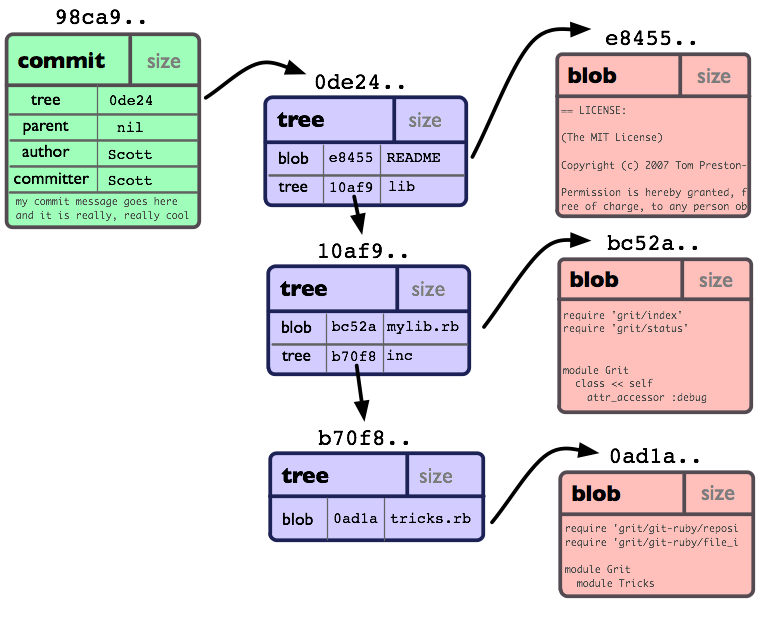
\includegraphics[width=7cm]{figs/objects-example.png}
  \end{center}

{\Tiny
Image from Git Community Book
(\url{http://book.git-scm.com/index.html})
}
\end{frame}

\section{Branching and Merging}

\begin{frame}[fragile]
  \frametitle{Working with branches}

  \begin{itemize}
  \item Branches are quite ``cheap'' (fast and clean process)
  \item Creating a new branch
    {\scriptsize
\begin{verbatim}
$ git branch <branch> [<start-point>]
\end{verbatim}
    }

  \item Listing available branches
    {\scriptsize
\begin{verbatim}
$ git branch
\end{verbatim}
    }

  \item Changing the current branch
    {\scriptsize
\begin{verbatim}
$ git checkout
\end{verbatim}
    }

  \item Creating a branch and changing to it in a single operation
    {\scriptsize
\begin{verbatim}
$ git checkout -b <branch> [<start-point>]
\end{verbatim}
    }      

  \item Merging branches
    {\scriptsize
\begin{verbatim}
$ git merge <branch>
\end{verbatim} 
    }

  \item Updating the current branch from another
    {\scriptsize
\begin{verbatim}
$ git rebase <branch>
\end{verbatim}
    }
  \end{itemize}
\end{frame}

\section{Operations between repositories}

\begin{frame}[fragile]
  \frametitle{Pulling}

  \begin{itemize}
  \item Cloning a repository (clone != checkout)
    {\scriptsize
\begin{verbatim}
$ git clone <uri>
\end{verbatim}
    }

  \item Getting updates
    {\scriptsize
\begin{verbatim}
$ git fetch <uri>
$ git merge origin/master
\end{verbatim}
    }

  \item Useful shortcut (commonly used)
    {\scriptsize
\begin{verbatim}
$ git pull
\end{verbatim}
    }

  \item Updating a remote repository
    {\scriptsize
\begin{verbatim}
$ git push
\end{verbatim}
    }

  \end{itemize}
\end{frame}

\begin{frame}[fragile]
  \frametitle{Workflow (Summary)}
  {\scriptsize
\begin{verbatim}
$ git clone <uri>
$ cd project
$ git checkout -b new-feature
(some changes, git add, etc.)
$ git commit -a
(more changes)
$ git commit -a
(last changes, my new feature is now ready)
$ git commit -a
$ git checkout master
$ git pull
$ git checkout new-feature
$ git rebase master
$ git checkout master
$ git merge new-feature
$ git push origin master
\end{verbatim}
  }
\end{frame}

\begin{frame}
  \frametitle{Big advantages for the daily work}

  \begin{itemize}
  \item Offline work
    \pause
  \item Working on more than one feature at the same time
    \pause
  \item Micro-commits
    \pause
  \item Easy sharing of code
    \pause
  \item Author != Committer
    \pause
  \item Better history
    \pause
  \item Interactivity with other systems (git-svn, git-cvs)
    \pause
  \item {\bf Performance!!!}
  \end{itemize}
\end{frame}

\begin{frame}[fragile]
  \frametitle{Some tips and tricks}

  \begin{itemize}
  \item Cherry-picking
    {\scriptsize
\begin{verbatim}
$ git cherry-pick <commit>
\end{verbatim}
    }

    \pause

  \item Move this away for a while, I need to fix something first
    {\scriptsize
\begin{verbatim}
$ git stash save "work in progress for foo thing"
changes, commit, push and whatever
$ git stash apply
\end{verbatim}
    }

    \pause

  \item Add chunks of files to the index
    {\scriptsize
\begin{verbatim}
$ git add file1 file2 ... filen --patch
\end{verbatim}
    }

  \end{itemize}
\end{frame}

\begin{frame}[fragile]
  \frametitle{Some tips and tricks}

  \begin{itemize}
  \item Append changes to last commit
    {\scriptsize
\begin{verbatim}
$ git commit --amend
\end{verbatim}
    }

    \pause

  \item Merge this, but please, do not change the history because I
    have some embarrassing private commits
    {\scriptsize
\begin{verbatim}
$ git merge --squash <branch>
$ git commit -a
$ git push
\end{verbatim}
    }

    \pause

  \item Looking for a regression
    {\scriptsize
\begin{verbatim}
$ git bisect start
$ git bisect good <commit-id>
$ git bisect bad <commit-id>
$ git bisect [good|bad]
(repeat until you find the guilty commit 
telling git if current version is good or bad)
$ git bisect reset
\end{verbatim}
    }
    \end{itemize}

\end{frame}

\begin{frame}[fragile]
  \frametitle{Patches}

  \begin{itemize}
  \item Creating series of patches
    {\scriptsize
\begin{verbatim}
$ git format-patch <commit-from>..<commit-to>
\end{verbatim}
    }

  \item Appliying series of patches
    {\scriptsize
\begin{verbatim}
$ cat patch1 patch2 .. patchn > patches.mbox
$ git am patches.mbox
\end{verbatim}
    }
    \end{itemize}

\end{frame}



%\section{Development Tools}

\section{GCC: The GNU Compiler Collection}

\begin{frame}
  \frametitle{Introduction}

  \begin{itemize}
  \item Originally named the GNU C Compiler, since it only handled
    the C programming language
  \item Today is a compiler system supporting various programming
    languages (C/C++, Java, ADA, Objective-C, Objective-C++, Fortran)
  \item Started by Richard Stallman in 1985
  \item Used in lots of platforms including embedded platforms
  \end{itemize}
\end{frame}

\begin{frame}[fragile]
  \frametitle{Compiling a C program}
\begin{verbatim}
$ gcc -g -Wall test.c -o test
\end{verbatim}
  Recommended flags
  \begin{itemize}
  \item -g: Produce debugging information
  \item -Wall: Turns on all optional warnings which are desirable for
    normal code
  \item -o: Write output to file
  \end{itemize}
\end{frame}

\begin{frame}[fragile]
  \frametitle{Compiling multi-file programs}

  One step
\begin{verbatim}
$ gcc -g -Wall -o test test-helper.c test.c
\end{verbatim}

  Compiling every file in a different step
\begin{verbatim}
$ gcc -g -Wall -c test-helper.c # test-helper.o
$ gcc -g -Wall -c test.c        # test.o
$ gcc -o test test-helper.o test.o
\end{verbatim}
\end{frame}

\begin{frame}[fragile]
  \frametitle{Linking}

  External libraries
\begin{verbatim}
$ gcc -o test test-helper.o test.o -lm
\end{verbatim}

  Library search path
  \begin{itemize}
  \item -Lpath
  \item Default: /usr/lib, /usr/local/lib
  \item Env variable: LD\_LIBRARY\_PATH
  \end{itemize}

  Include search path
  \begin{itemize}
  \item -Ipath
  \item Default: /usr/include /usr/local/include
  \item Env variable: C\_INCLUDE\_PATH
  \end{itemize}
\end{frame}

\begin{frame}
  \frametitle{Static and Shared libraries}

  \begin{itemize}
  \item Static: included into the binary executable (in UNIX .a)
  \item Dynamic: loaded into the program at runtime (in UNIX .so)
  \end{itemize}

  Dynamic libraries are the default option when available. The static
  linking can be forced by using the --static flag when compiling with
  gcc.
\end{frame}

\begin{frame}
  \frametitle{pkg-config: metainformation about installed libraries}

  Common options used for compiling
  \begin{itemize}
  \item --cflags: prints pre-processor and compile flags required to
    compile
  \item --libs: prints the link flags
  \end{itemize}

  Options to get information about a library
  \begin{itemize}
  \item --modversion: prints the version of the installed library
  \item --exists
  \item --atleast-version=VERSION
  \item --exact-version=VERSION
  \item --max-version=VERSION
  \end{itemize}

  Option to get the list of installed libraries
  \begin{itemize}
  \item --list-all
  \end{itemize}
\end{frame}

\section{Automatic building}

\begin{frame}[fragile]
  \frametitle{Makefile}

  \begin{itemize}
  \item Text file used by the make command
  \item Consists of rules with the following shape:
\begin{verbatim}
target: dependencies
    commands
\end{verbatim}

    \begin{itemize}
    \item target: the name of an output file or another action to be
      carried out
    \item dependencies: target prerequisites needed to run the command
    \item commands: action that is finally carried out
    \end{itemize}

  \item Once the Makefile is created we can run the make command
\begin{verbatim}
$ make target
\end{verbatim}
  \item By default, make starts with the first target. 
  \end{itemize}
\end{frame}

\begin{frame}[fragile]
  \frametitle{Writing Makefiles}
  \begin{itemize}
  \item We can use variables like in a shell script with \$(variable)
  \item Wildcard characters ('*', '?' and '[..]' like in bash)
  \item Pattern Rules (with \% character)
\begin{verbatim}
$ target: target-pattern: prereq-patterns
    commands
\end{verbatim}
  \item Some special variables
    \begin{itemize}
    \item \$@: current target name
    \item \$<: first prerequisite of the current rule
    \item \$\^~: the list of prerequisites of the current rule
    \item \$+: the list of prerequisites of the current rule including
      duplicates
    \item \$?: the list of prerequisites that are newer than the target
    \end{itemize}

  \end{itemize}
\end{frame}

\begin{frame}
  \frametitle{GNU Autotools}
  Set of tools for creating a building system for a software package
  \begin{itemize}
  \item Autoconf: produces shell scripts that automatically configure
    software source code packages
  \item Automake: produces Makefile.in files 
  \item Libtool: creates portable libraries
  \item Gettext: internationalization 
  \end{itemize}
\end{frame}

\begin{frame}
  \frametitle{Autoconf}
  \begin{itemize}
  \item Scripts generated by autoconf don't depend on autoconf to be run
  \item Based on macros and templates it generates a configure script
    suitable for you software package which doesn't need any further
    modification
  \item Autoconf creates the configure script by using another script written by
    the user (commonly named configure.ac or configure.in)
  \item And finally the configure script converts Makefile.in files
    into final Makefiles that can be processed with make
  \item In order to create a complete and portable build system
    autoconf should be used in combination with other tools like Automake
  \end{itemize}
\end{frame}

\begin{frame}
  \frametitle{Automake}
  \begin{itemize}
  \item Creates Makefile.in files from Makefile.am files written by
    the user.
  \item It makes writing Makefiles easier and simpler
  \item Automatically generates dependencies so that files are not
    always recompiled, but only when they have changed
  \end{itemize}
\end{frame}

\begin{frame}[fragile]
  \frametitle{pkg-config: Autoconf macros}
{\tiny
\begin{verbatim}
  PKG_CHECK_MODULES(VARIABLE-PREFIX,MODULES[,ACTION-IF-FOUND,[ACTION-IF-NOT-FOUND]])
\end{verbatim}
}
\begin{itemize}
\item The most commonly used pkg-config Autoconf macro
\item Checks whether a module exists
\item Generates \_CFLAG and \_LIBS substitution variables, set to the
  libs and cflags for the given module list
\item Default action is to abort when a module is not found or has
  wrong version
\end{itemize}
{\tiny
\begin{verbatim}
PKG_CHECK_MODULES([MY_PROJECT], [glib-2.0 >= 2.1.5 libxml-2.0 >= 2.0.0])
\end{verbatim}
}
\end{frame}

\begin{frame}[fragile]
  \frametitle{Hello world example: configure.ac}
\begin{verbatim}
dnl Process this file with autoconf to produce 
dnl a configure script.

AC_INIT([hello], [0.1])

AM_INIT_AUTOMAKE([1.9])
AC_PROG_CC
AC_CONFIG_HEADERS([config.h])
AC_CONFIG_FILES([
Makefile
src/Makefile
])
AC_OUTPUT
\end{verbatim}
\end{frame}

\begin{frame}[fragile]
  \frametitle{Hello world example: Makefiles}
  Makefile.am
\begin{verbatim}
SUBDIRS=src
\end{verbatim}
  src/Makefile.am
\begin{verbatim}
bin_PROGRAMS=hello
hello_SOURCES=main.c
\end{verbatim}

\end{frame}

\begin{frame}[fragile]
  \frametitle{Hello world with dependencies example: configure.ac}
{\scriptsize
\begin{verbatim}
dnl Process this file with autoconf to produce 
dnl a configure script.

AC_INIT([hello], [0.1])

AM_INIT_AUTOMAKE([1.9])
AC_PROG_CC
AM_PROG_CC_C_O
AC_CONFIG_HEADERS([config.h])

PKG_CHECK_MODULES([HELLO], [glib-2.0])
AC_SUBST(HELLO_CFLAGS)
AC_SUBST(HELLO_LIBS)

AC_CONFIG_FILES([
Makefile
src/Makefile
])
AC_OUTPUT
\end{verbatim}
}
\end{frame}

\begin{frame}[fragile]
  \frametitle{Hello world with dependencies example: Makefiles}

  src/Makefile.am
\begin{verbatim}
bin_PROGRAMS=hello
hello_SOURCES=main.c
hello_CPPFLAGS=$(HELLO_CFLAGS)
hello_LDADD=$(HELLO_LIBS)
\end{verbatim}
\end{frame}


%\section{Django}

\begin{frame}
\frametitle{Introduction to Django}
\begin{itemize}
\item Web development framework
\item Provides a set of resources for creating complex web applications 
  in an easy way
\item Development based on Python programming language and the
 Model-View-Controller pattern (MVC)
\item Open Source Project (BSD License)
\item \url{http://www.djangoproject.com}
\end{itemize}
\end{frame}

\begin{frame}
\frametitle{Model-View-Controller Pattern (MVC) (i)}
\begin{center}
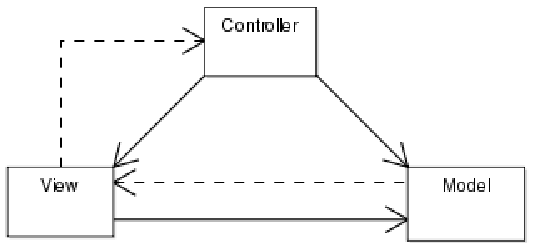
\includegraphics[width=10cm]{figs/MVC}
\end{center}
\end{frame}


\begin{frame}
\frametitle{Model-View-Controller Pattern (MVC) (ii)}
\begin{itemize}
\item \textbf{Model}: Representation of the data on which the application operates (raw data)
\item \textbf{View}: User interface
\item \textbf{Controller}: Manages the users requests and acts as exchanger between the model
  and the views.
\end{itemize}
\end{frame}


\begin{frame}[fragile]
\frametitle{Starting a Project}
\begin{itemize}
\item A \textbf{project} is a collection of settings for an instance of Django, including
  database configuration, Django-specific-options, and application-specific
  settings (\textit{Django Book})
\item An \textbf{application} is a portable set of Django functionality, 
   usually including models and views, that lives together in a single 
   Python package.
\item Initial commands
{\scriptsize
\begin{verbatim}
  django-admin.py startproject <PROJECT>
  django-admin.py startapp <APP>
  manage.py runserver [DOMAIN]
\end{verbatim}
}
\end{itemize}
\end{frame}


\begin{frame}
\frametitle{Introduction to DB Model}
\begin{itemize}
\item Data access layer
\item Supports several database storage engines (MySQL, PostgreSQL, SQLite, Oracle)
\item Access based on an ORM (Object Relational Mapper)
\item Suitable for object-programming 
\end{itemize}
\end{frame}


\begin{frame}[fragile]
\frametitle{Database Configuration}
\begin{itemize}
\item settings.py
{\scriptsize
\begin{verbatim}
  DATABASE_ENGINE = ""
  DATABASE_NAME = ""
  DATABASE_USER = ""
  DATABASE_PASSWORD = ""
  DATABASE_HOST = ""
  DATABASE_PORT = ""
\end{verbatim}
}
\end{itemize}
\end{frame}


\begin{frame}[fragile]
\frametitle{Useful DB commands }
\begin{itemize}
\item Validate model
{\scriptsize
\begin{verbatim}
  python manage.py validate
\end{verbatim}
}
\item Generate SQL
{\scriptsize
\begin{verbatim}
  python manage.py sqlall <app>
\end{verbatim}
}
\item Synchronize Model
{\scriptsize
\begin{verbatim}
  python manage.py syncdb
\end{verbatim}
}
\end{itemize}
\end{frame}


\begin{frame}[fragile]
\frametitle{Defining the Model}
\begin{itemize}
\item All classes inherit from models.Model
{\scriptsize
\begin{verbatim}
from django.db import models
   
class Author(models.Model):
  name = models.CharField(max_length=50)
  email = models.EmailField()
\end{verbatim}
}
\end{itemize}
\end{frame}


\begin{frame}[fragile]
\frametitle{Model Fields}
{\scriptsize
\begin{verbatim}
 - AutoField
 - CharField
 - TextField
 - IntegerField
 - FloatField
 - DateTimeField
 - BooleanField
\end{verbatim}
}
\end{frame}


\begin{frame}[fragile]
\frametitle{Model Relationships}
{\scriptsize
\begin{verbatim}
  ForeignKey(othermodel) -> 1-N
    a.fk = b
  OneToOneField(othermodel) -> 1-1 (FK with unique=True)
    a.fk = b
  ManyToManyField(othermodel) -> N-N
    a.fk.add(b)
\end{verbatim}
}
\end{frame}


\begin{frame}[fragile]
\frametitle{Model Field options}
{\scriptsize
\begin{verbatim}
  null=Boolean
  default=Type
  primary_key=Boolean
  unique=Boolean
  unique_for_date=Boolean
\end{verbatim}
}
\end{frame}

\begin{frame}[fragile]
\frametitle{Dealing with Model objects}
\begin{itemize}
\item Creating
{\scriptsize
\begin{verbatim}
a = Author(name='sduenas', ...)
a.save()
\end{verbatim}
}
\item Updating attributes
{\scriptsize
\begin{verbatim}
a.name = 'carlosgc'
a.save()
\end{verbatim}
}
\item Deleting
{\scriptsize
\begin{verbatim}
a.delete()
\end{verbatim}
}
\end{itemize}
\end{frame}

\begin{frame}[fragile]
\frametitle{Searching}
\begin{itemize}
\item Basic search
{\scriptsize
\begin{verbatim}
Author.objects.all()
Author.objects.get()
\end{verbatim}
}
\item Filters
{\scriptsize
\begin{verbatim}
Author.objects.filter(name="")
Author.objects.filter(name="Jesus", email__contains="libresoft.es")
Author.objects.order_by("name", "-email")
Author.objects.filter(name="").order_by("name")
\end{verbatim}
}
\end{itemize}
\end{frame}


%*********************************************************************
%*********************************************************************
%*********************************************************************

%\section{URLconfs}

\begin{frame}[fragile]
\frametitle{Introduction to URLconfs}
\begin{itemize}
\item Regular Expressions
\item Map URL patterns to views
{\scriptsize
\begin{verbatim}
from django.conf.urls.defaults import *

urlpatterns = patterns("",
  (r"^mysite/", include("mysite.urls")),
  (r"^admin/", include("django.contrib.admin.urls")),
)
\end{verbatim}
}
\end{itemize}
\end{frame}


\begin{frame}
\frametitle{Regular Expressions}
\begin{table}
\begin{small}
\centering
\begin{tabular}{|c|l|}
\hline
\textbf{Symbol} & \textbf{Meaning} \\
\hline
 . (dot) & any char \\
\hline
 * (dot) & 0 or more previous chars \\
\hline
 + (dot) & 1 or more previous chars \\
\hline
 ? (dot) & 0 or 1 previous char \\
\hline
 (?P<p>) & group and parameter \\
\hline
 [] & set of chars \\
\hline
{min,max} & range \\
\hline
\end{tabular}
\end{small}
\end{table}
\end{frame}


\begin{frame}[fragile]
\frametitle{URLconf Example}
{\scriptsize
\begin{verbatim}
 urlpatterns = patterns("",
   (r"^id/(?P<name>[A-Za-z\-]+)$", "mysite.views.id"),
   (r"^id/(?P<name>[A-Za-z\-]+)/auth/(?P<type>[a-z]+)$",
           "mysite.views.auths"),
   (r"^/num/(?P<num>d{2})$", "mysite.views.id"),
   (r"(?P<path>.*)$", "django.views.static.serve", 
      {"document_root": "/var/www/myproject/"},
 )
\end{verbatim}
}
\end{frame}


%*********************************************************************
%*********************************************************************
%*********************************************************************


\begin{frame}[fragile]
\frametitle{Views}
\begin{itemize}
\item Render template
{\scriptsize
\begin{verbatim}
render_to_response(<template>, <dict>)
\end{verbatim}
}
\item HttpResponse
{\scriptsize
\begin{verbatim}
HttpResponse(response, mimetype=<type>)
\end{verbatim}
}
\end{itemize}
\end{frame}

\begin{frame}[fragile]
\frametitle{Templates}
\begin{itemize}
\item Produce a dynamic text output requested by the user
\item Composed by text, variables (\{\{ var \}\}) and tags (\{\% tag \% \})
\item Context variables are passed from the view dictionary
\item Template and Context objects is also available
\end{itemize}
\end{frame}


\begin{frame}[fragile]
\frametitle{Tags (i)}
\begin{itemize}
\item \textit{if/else}
{\scriptsize
\begin{verbatim}

   <p>Found</p>

   <p>Not found</p>

\end{verbatim}
}
\item \textit{for}
{\scriptsize
\begin{verbatim}

   <p>{{day}}</p>

\end{verbatim}
}
\end{itemize}
\end{frame}


\begin{frame}[fragile]
\frametitle{Tags (ii)}
\begin{itemize}
\item \textit{include}
{\scriptsize
\begin{verbatim}

\end{verbatim}
}
\item \textit{block}
{\scriptsize
\begin{verbatim}

   <h1>Title</h1>

\end{verbatim}
}
\item \textit{extends}
{\scriptsize
\begin{verbatim}

\end{verbatim}
}
\end{itemize}
\end{frame}


%\section{More Django}

\begin{frame}
\frametitle{More on Django}
\begin{itemize}
\item Administration Site
\item Forms
\item Template Engine Extensions
\end{itemize}
\end{frame}


%\section{References}

\begin{frame}
\frametitle{References}
\begin{itemize}
\item \textit{Django Book} \url{http://www.djangobook.com/}
\item \textit{Django Documentation} \url{http://docs.djangoproject.com/en/dev/}
\end{itemize}
\end{frame}



\end{document}

